\chapternotnumbered{Precautions} \label{ch:precautions}

Before working with any Digifiz Replica dashboard, review and follow the following safety notes.
Most damage reported in the field is caused by overlooking one of these rules.

\begin{enumerate}
    \item Disconnect the vehicle battery before removing the original cluster or connecting any Digifiz instrument panel.
          Leaving the harness powered during installation has destroyed several dashboards.
    \item Never apply an external supply voltage---even through a current-limiting resistor---to the sensor inputs (outside temperature, oil temperature, coolant temperature, or fuel level).
          These inputs are designed for passive sensors and are permanently damaged by active sources.
    \item Generation~1 and 1.5 dashboards do not contain internal fuses.
          The first protective element is the vehicle fuse rated at 15~A, which is too high to protect the panel electronics.
    \item Protect the instrument cluster from direct sunlight.
          Prolonged exposure significantly reduces display contrast.
    \item The LED backlight used in Generations~1, 1.5, and 2 cannot be overdriven to increase brightness.
          Shield the cluster from direct light if the display is difficult to read.
    \item Mechanical cable speedometer drives may resonate at 40--60~km/h, producing unstable readings.
          Install the supplied electronic drive whenever possible---it ships with all current Gen~1.5 and Gen~2 panels.
    \item Generation~2 panels omit the touch sensor located behind the VW badge.
          MFA modes must be controlled from an external switch on these units.
    \item The Generation~2 design draws 11--13~mA from the vehicle battery in standby.
          This quiescent load cannot be reduced and should be considered when the car is parked for several months.
    \item None of the instrument cluster variants ship with an instantaneous fuel consumption display.
          The feature can be retrofitted to Gen~1 and Gen~1.5 panels using the instructions at\newline\url{https://www.youtube.com/watch?v=qWqvYc9388U}; the upgrade has not been validated on Gen~2 units.
\end{enumerate}

\begin{figure}[htbp]
    \centering
    \begin{subfigure}{0.45\textwidth}
        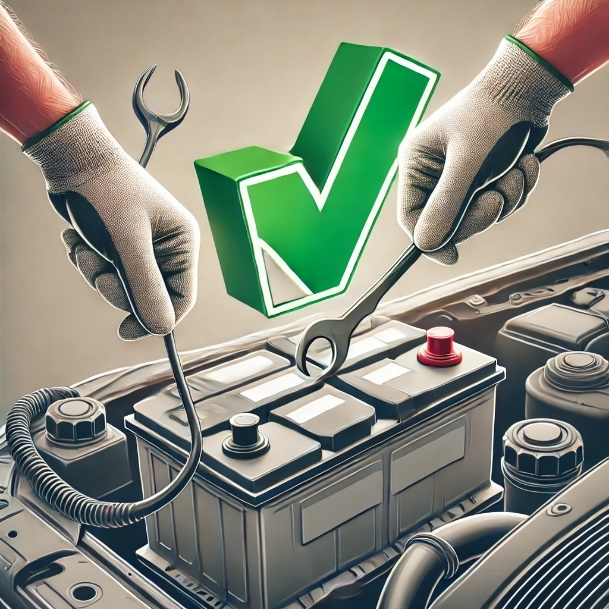
\includegraphics[width=\linewidth]{digifiz_manual/image001.jpg}
        \caption{Reminder to disconnect the battery before servicing.}
    \end{subfigure}\hfill
    \begin{subfigure}{0.45\textwidth}
        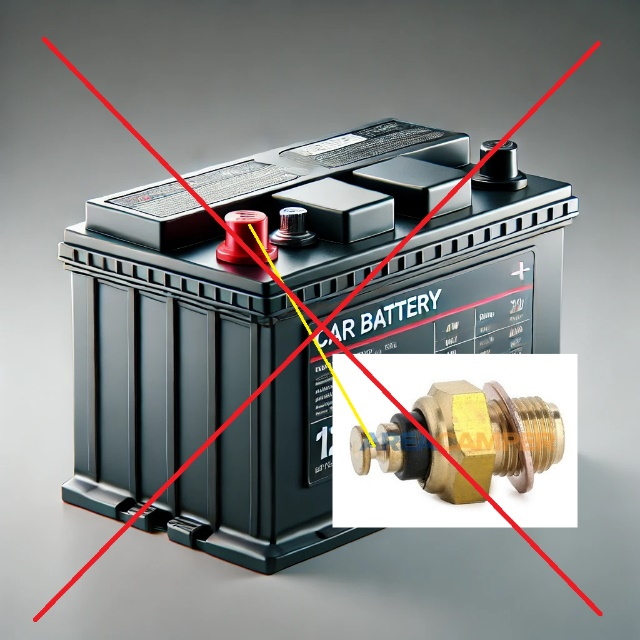
\includegraphics[width=\linewidth]{digifiz_manual/image002.jpg}
        \caption{Warning about applying external voltage to sensor circuits.}
    \end{subfigure}
    \caption{Typical warning labels supplied with the wiring harness.}
\end{figure}

Treat the dashboards as precision electronics: avoid ESD, moisture, and mechanical shock, and never use sensor readings for automated vehicle control.
